\documentclass[a4paper]{article}
\usepackage{fancyhdr}
\usepackage[includeheadfoot,left=1in, right=0.5in, top=0.5in, bottom=0.5in]{geometry}
\usepackage{lastpage}
\usepackage{extramarks}
\usepackage[usenames,dvipsnames]{color}
\usepackage{graphicx}
\usepackage{listings}
\usepackage{courier}
\usepackage{tikz}
\usepackage{color}
\usepackage{float}
\usepackage{url}
\usepackage{subfigure}
\usepackage{varwidth}
\usepackage{caption}
\usepackage{multirow}
\usepackage[pdfborder={0 0 0}]{hyperref}
\usepackage[compact,small]{titlesec}
\usepackage{microtype}
\usepackage{verbatim}
\usepackage{booktabs}
\usepackage{indentfirst}
\usepackage{enumitem}
\usepackage{pdfpages}

\captionsetup[sub]{labelsep=newline}

% line spacing
\linespread{1.0}

% bold item
\let\origitem\item
\renewcommand{\item}{\normalfont\origitem}
\newcommand{\bolditem}{\small\bfseries\origitem}

% tilde
%\newcommand{\small_tilde}{\raise.17ex\hbox{$\scriptstyle\sim$}}

% indent item
\newcommand{\indentitem}{\setlength\itemindent{24pt}}

\parskip = 0.5\baselineskip
\setlength{\belowcaptionskip}{-\baselineskip}

\captionsetup{font=scriptsize}
\captionsetup{labelfont=bf}

\pagestyle{fancy}
\rhead{Samir Silbak \& Manasa Kasula}
\lhead{EECE6080 - Project}
\rfoot{Page\ \thepage\ of \protect\pageref{LastPage}}
\cfoot{}
\renewcommand\headrulewidth{0.4pt}
\renewcommand\footrulewidth{0.4pt}

% make verbatim text small
\makeatletter
\g@addto@macro\@verbatim\small
\makeatother

\setlength\parindent{0pt} % Removes all indentation from paragraphs
%\setlength\parindent{24pt}

\definecolor{sh_comment}{rgb}{0.12, 0.38, 0.18 } %adjusted, in Eclipse: {0.25, 0.42, 0.30 } = #3F6A4D
\definecolor{sh_keyword}{rgb}{0.37, 0.08, 0.25}  % #5F1441
\definecolor{sh_string}{rgb}{0.06, 0.10, 0.98} % #101AF9

%\sectionfont{\centering}
\lstset{
    language=vhdl,
    xleftmargin=.25in,
    xrightmargin=.25in,
    numbers=left,
    numberstyle=\tiny,
    frame=tb,
    showstringspaces=false,
    captionpos=b,
    stringstyle=\color{sh_string},
    keywordstyle = \color{sh_keyword}\bfseries,
    commentstyle=\color{sh_comment}\itshape,
    basicstyle=\small\sffamily,
    %numbersep=-5pt,
    belowskip=\baselineskip,
    aboveskip=\baselineskip
}
\usepackage{authblk}

\title{
    \vspace{2in}
    \textbf{VLSI \\}
    \vspace{10pt}
    \textbf{PROGRAMMABLE BINARY TREE COMPUTATION\\}
    \vspace{10pt}
    \textbf{CHIP NAME: PBTCKS}
    \vspace{2in}
}

\author[1]{Samir Silbak}
\author[2]{Manasa Kasula}

\affil[1]{silbaksr@mail.uc.edu}
\affil[2]{kasulama@mail.uc.edu
    \vspace{10pt}
}
\affil[1]{(513) 207-0687}
\affil[2]{(847) 612-7364
    \vspace{2.0in}
}
\titleformat*{\section}{\large\normalfont}

\begin{document}

%\includepdf{}
\maketitle
\newpage
\parskip = 0.2\baselineskip
\newpage
\tableofcontents
\newpage
\listoffigures
\listoftables
\lstlistoflistings
\parskip = 0.5\baselineskip
\newpage
\input{../progress_1/progress_1_body.tex}
\newpage

\section{\textbf{Magic Layouts}}

\subsection{\textbf{LUT Slice Layout}}
    \begin{figure}[H]
        \centering
        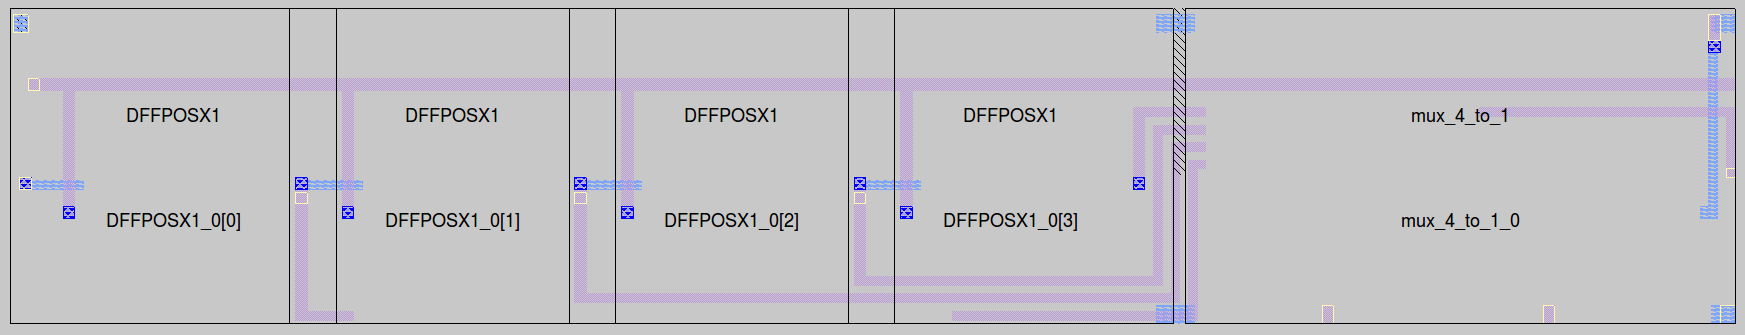
\includegraphics[width=\textwidth,height=\textheight,keepaspectratio]{../../magic/pics/lut_slice.png}
        \caption{\textbf{LUT Slice Magic Layout}}
        \label{fig:gg}
    \end{figure}
    \begin{figure}[H]
        \centering
        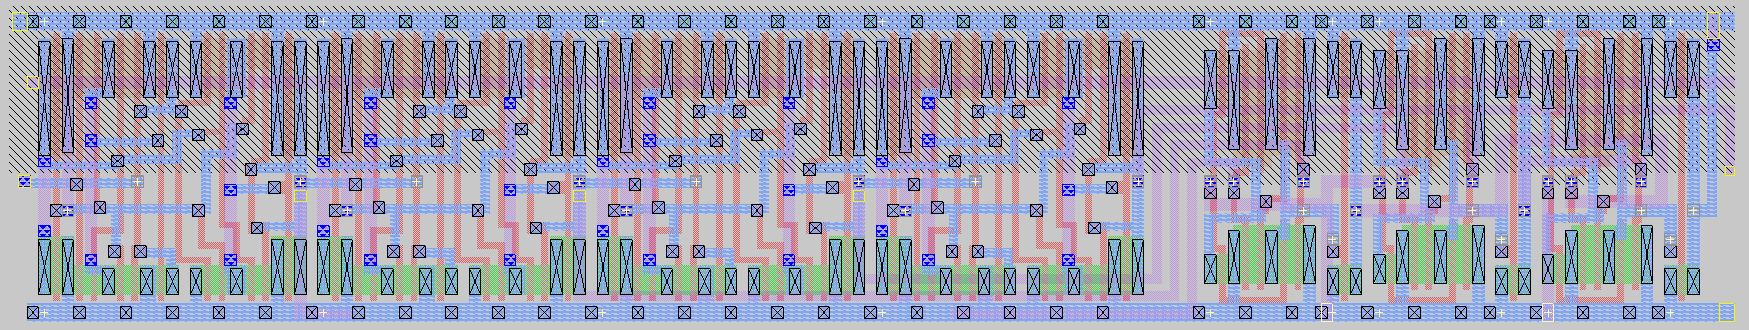
\includegraphics[width=\textwidth,height=\textheight,keepaspectratio]{../../magic/pics/lut_slice_internal.png}
        \caption{\textbf{LUT Slice Internal Magic Layout}}
        \label{fig:gg}
    \end{figure}

\subsection{\textbf{Shift Slice Layout}}
    \begin{figure}[H]
        \centering
        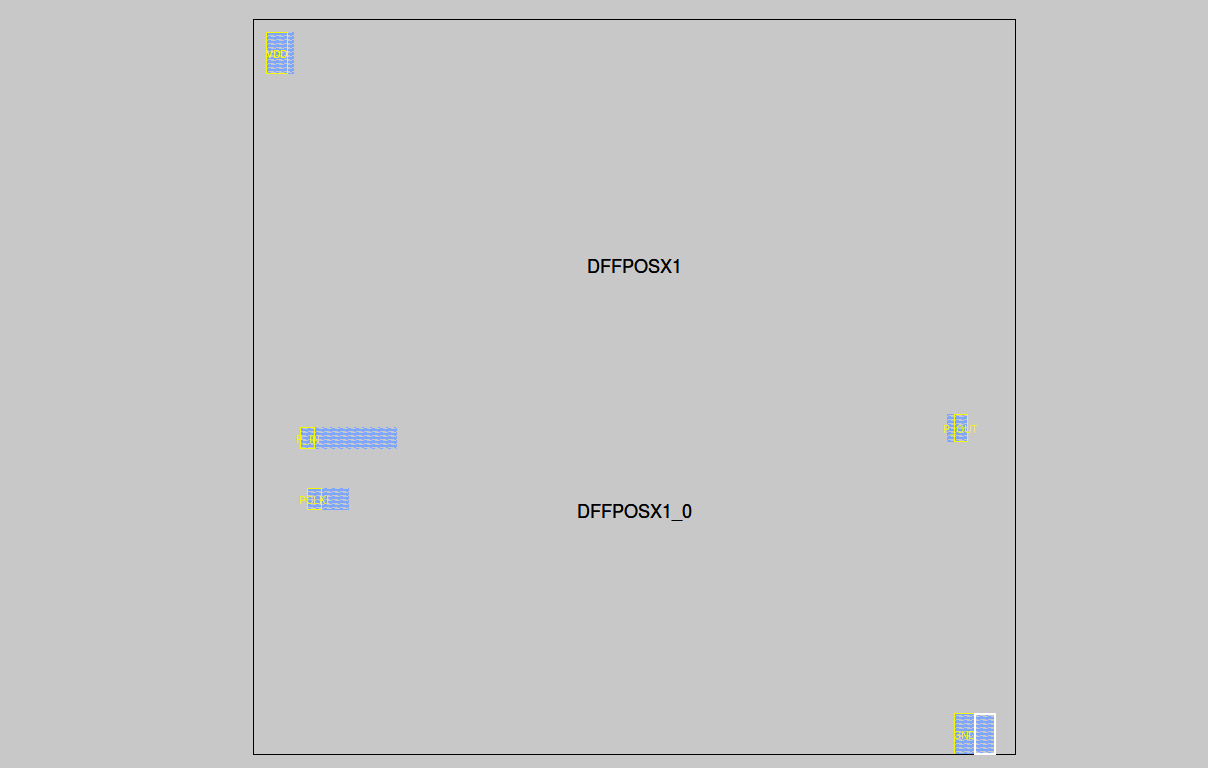
\includegraphics[width=\textwidth,height=\textheight,keepaspectratio]{../../magic/pics/shift_slice.png}
        \caption{\textbf{Shift Slice Magic Layout}}
        \label{fig:gg}
    \end{figure}
    \begin{figure}[H]
        \centering
        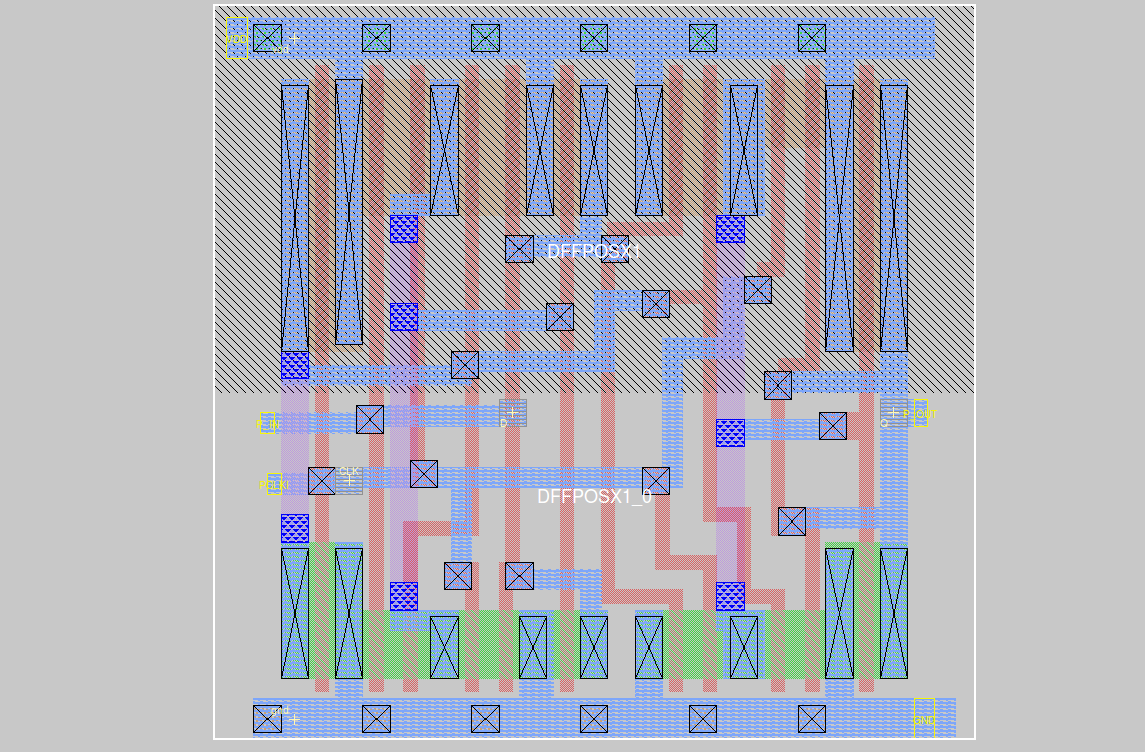
\includegraphics[width=\textwidth,height=\textheight,keepaspectratio]{../../magic/pics/shift_slice_internal.png}
        \caption{\textbf{Shift Slice Internal Magic Layout}}
        \label{fig:gg}
    \end{figure}

\section{\textbf{IRSIM Simulations}}
\subsection{\textbf{Bit Slice Simulations}}
    \begin{figure}[H]
        \centering
        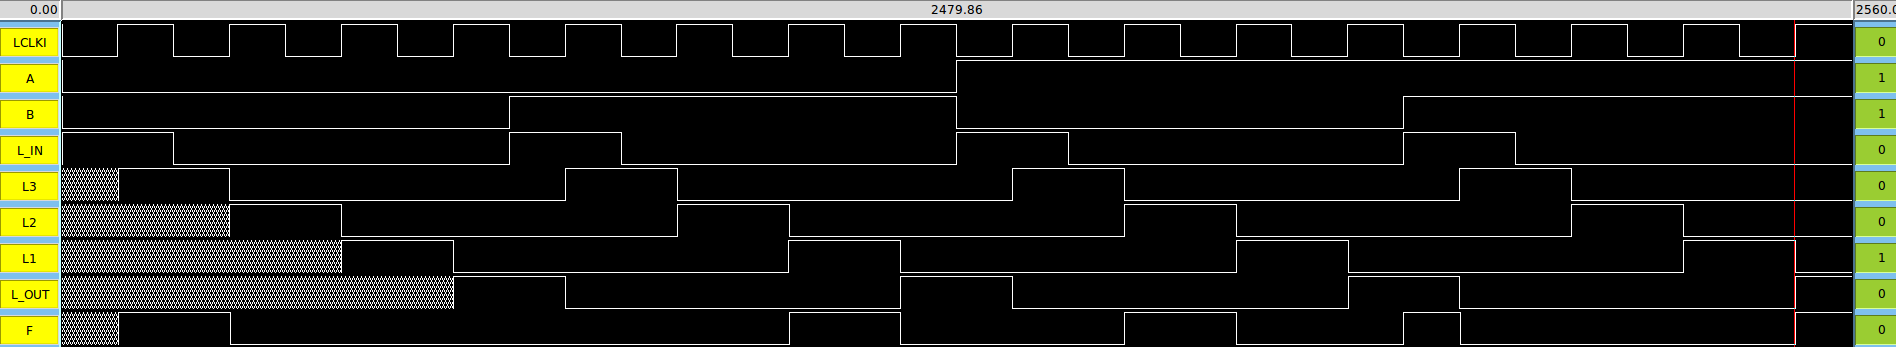
\includegraphics[width=\textwidth,height=\textheight,keepaspectratio]{../../irsim/pics/lut_and_ab.png}
        \caption{\textbf{LUT Slice with AND gate 'programmed'}}
        \label{fig:gg}
    \end{figure}
    %\begin{figure}[H]
    %    \centering
    %    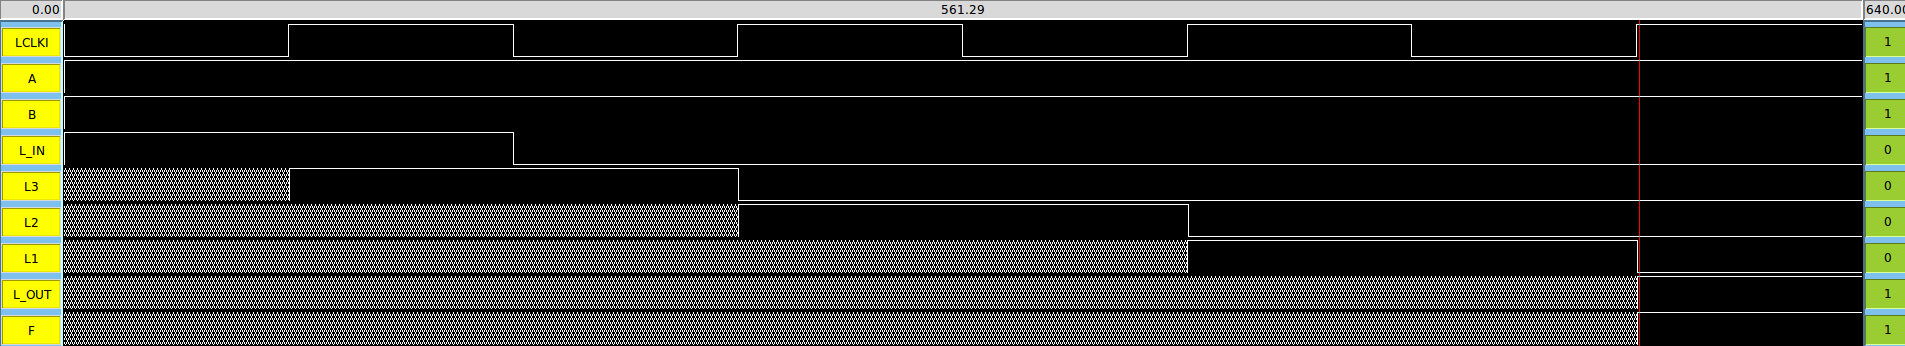
\includegraphics[width=\textwidth,height=\textheight,keepaspectratio]{../../irsim/pics/lut_and_fn.png}
    %    \caption{\textbf{LUT Slice with AND gate 'programmed'}}
    %    \label{fig:gg}
    %\end{figure}
    \begin{figure}[H]
        \centering
        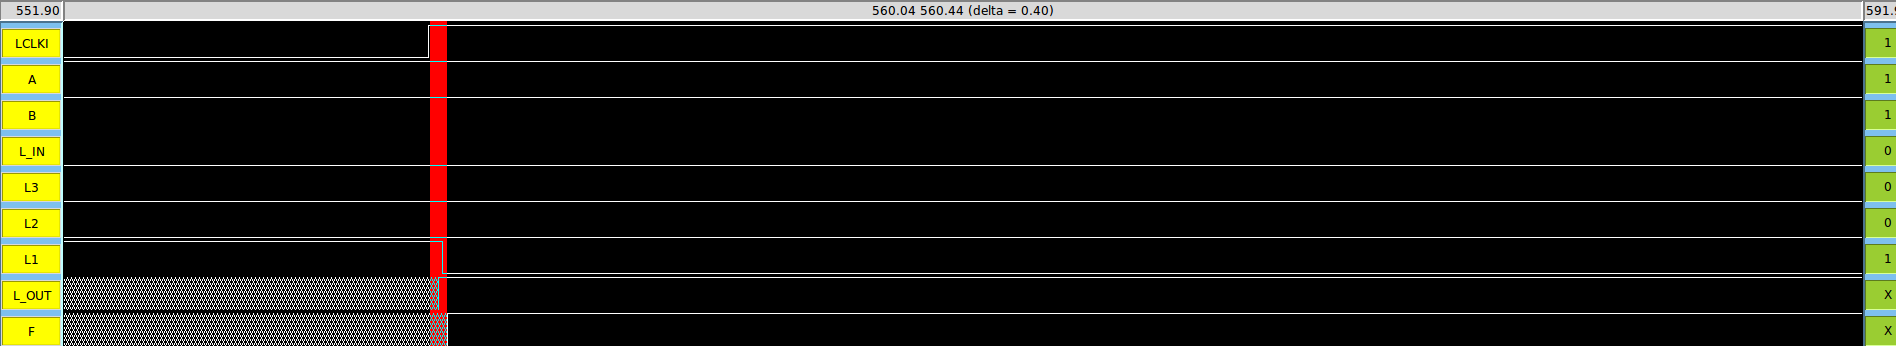
\includegraphics[width=\textwidth,height=\textheight,keepaspectratio]{../../irsim/pics/lut_f_rising.png}
        \caption{\textbf{Rising Edge of F output of LUT Slice}}
        \label{fig:gg}
    \end{figure}
    \begin{figure}[H]
        \centering
        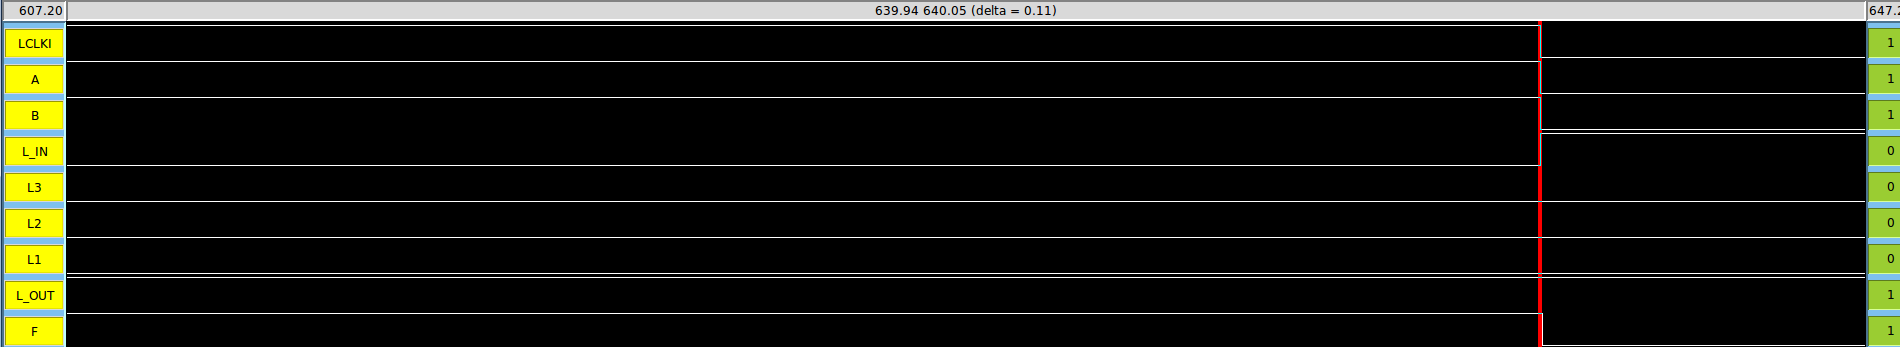
\includegraphics[width=\textwidth,height=\textheight,keepaspectratio]{../../irsim/pics/lut_f_falling.png}
        \caption{\textbf{Falling Edge of F output of LUT Slice}}
        \label{fig:gg}
    \end{figure}
    \begin{figure}[H]
        \centering
        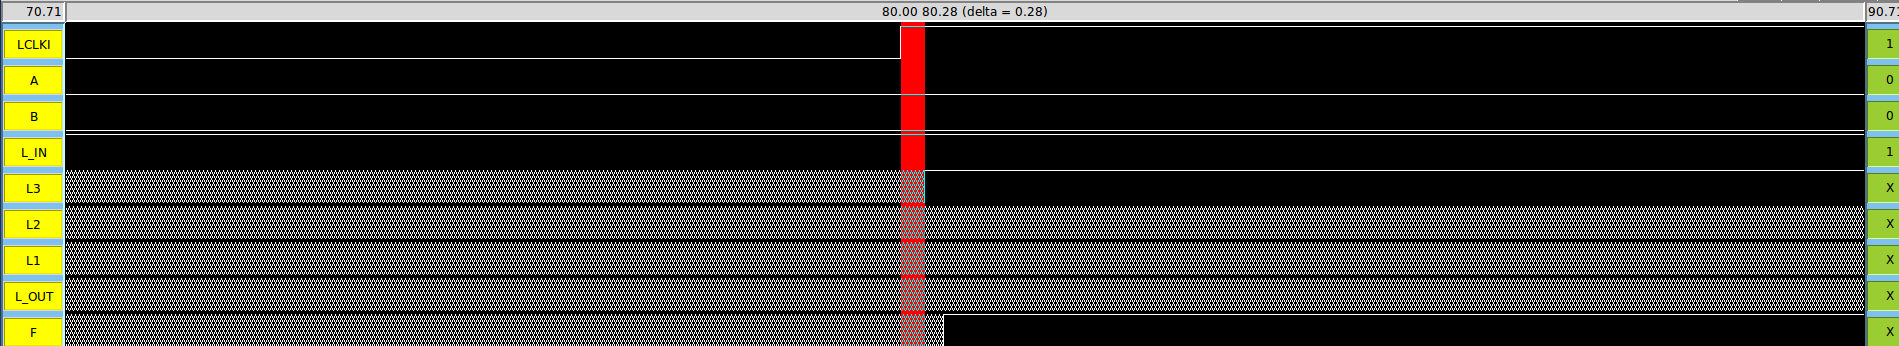
\includegraphics[width=\textwidth,height=\textheight,keepaspectratio]{../../irsim/pics/lut_l3_rising.png}
        \caption{\textbf{Rising Edge of L3 DFF of LUT Slice}}
        \label{fig:gg}
    \end{figure}
    \begin{figure}[H]
        \centering
        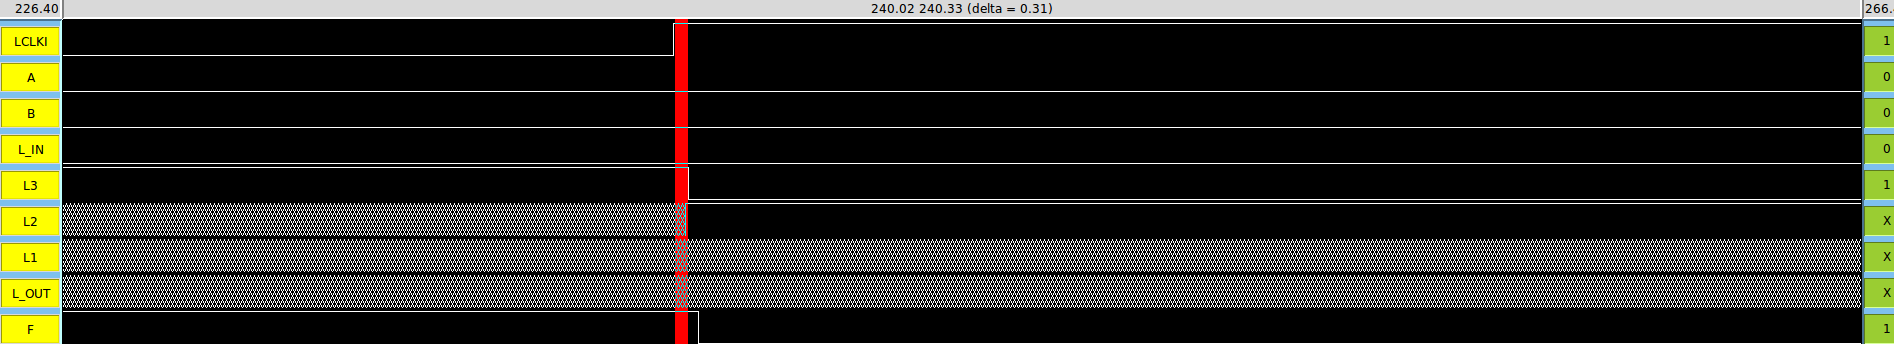
\includegraphics[width=\textwidth,height=\textheight,keepaspectratio]{../../irsim/pics/lut_l3_falling.png}
        \caption{\textbf{Falling Edge of L3 DFF of LUT Slice}}
        \label{fig:gg}
    \end{figure}

    \begin{figure}[H]
        \centering
        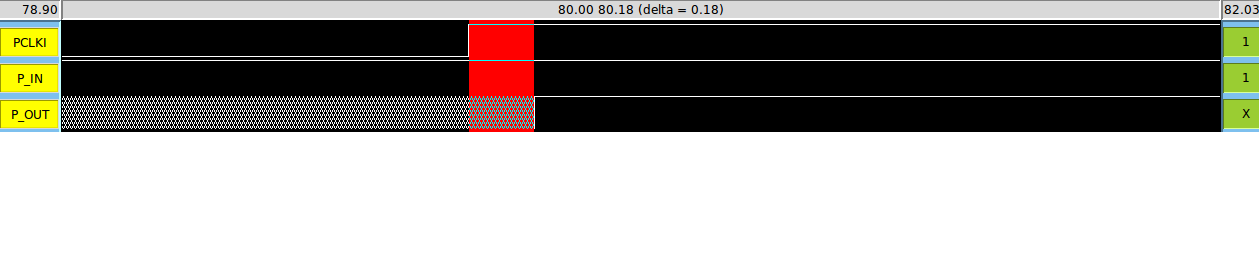
\includegraphics[width=\textwidth,height=\textheight,keepaspectratio]{../../irsim/pics/shift_rising.png}
        \caption{\textbf{Rising Edge of DFF of Shift Slice}}
        \label{fig:gg}
    \end{figure}
    \begin{figure}[H]
        \centering
        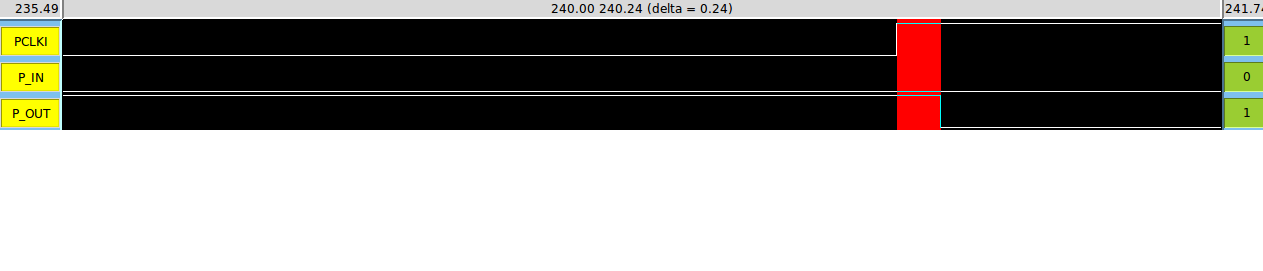
\includegraphics[width=\textwidth,height=\textheight,keepaspectratio]{../../irsim/pics/shift_falling.png}
        \caption{\textbf{Falling Edge of DFF of Shift Slice}}
        \label{fig:gg}
    \end{figure}
    \begin{figure}[H]
        \centering
        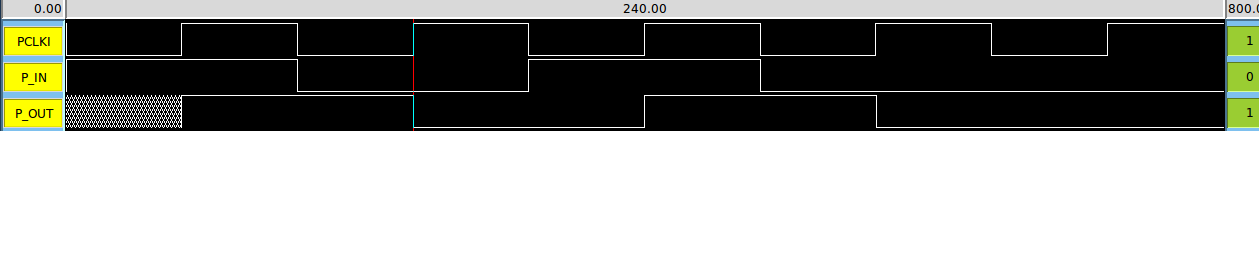
\includegraphics[width=\textwidth,height=\textheight,keepaspectratio]{../../irsim/pics/shift_waveform.png}
        \caption{\textbf{Waveform of DFF of Shift Slice}}
        \label{fig:gg}
    \end{figure}

\section{\textbf{Gate Level Simulations}}
    \begin{figure}[H]
        \centering
        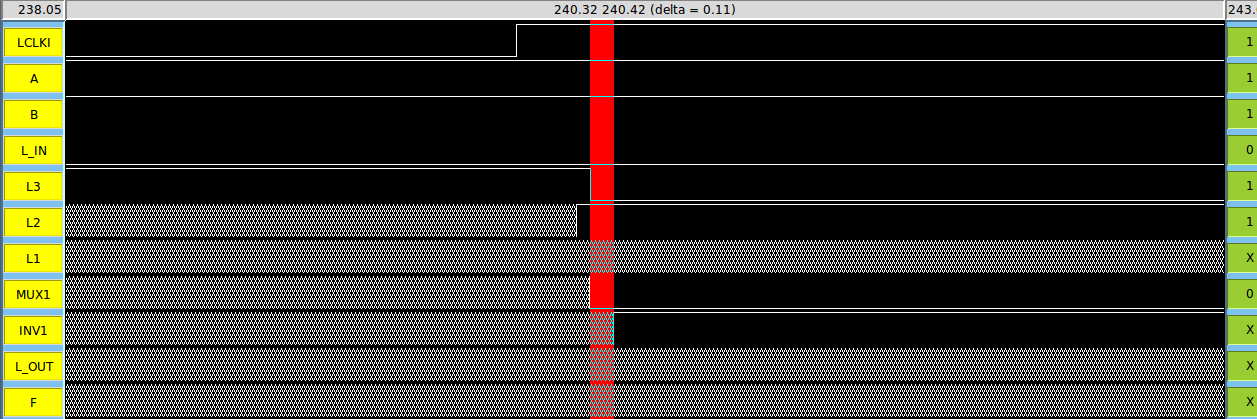
\includegraphics[width=\textwidth,height=\textheight,keepaspectratio]{../../irsim/pics/inv_rising.png}
        \caption{\textbf{Rising Edge of Inverter}}
        \label{fig:gg}
    \end{figure}
    \begin{figure}[H]
        \centering
        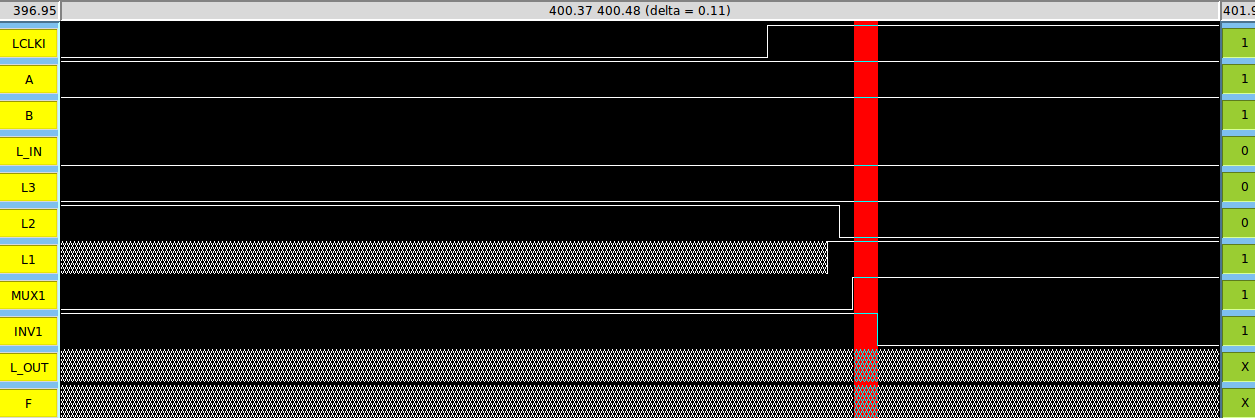
\includegraphics[width=\textwidth,height=\textheight,keepaspectratio]{../../irsim/pics/inv_falling.png}
        \caption{\textbf{Falling Edge of Inverter}}
        \label{fig:gg}
    \end{figure}
    \begin{figure}[H]
        \centering
        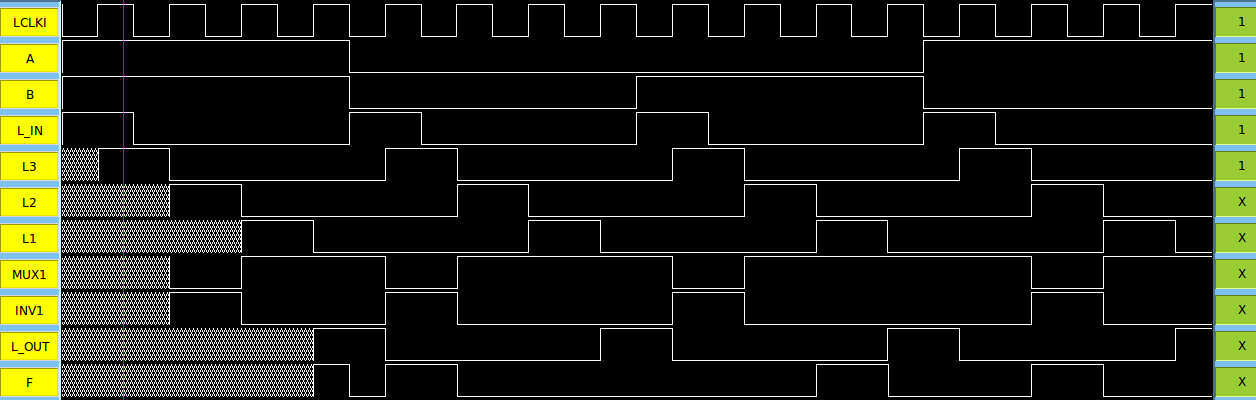
\includegraphics[width=\textwidth,height=\textheight,keepaspectratio]{../../irsim/pics/inv_waveform.png}
        \caption{\textbf{Waveform of LUT Slice (Includes nodes at each flip flop)}}
        \label{fig:gg}
    \end{figure}

\section{\textbf{HSpice Simulations}}
\subsection{\textbf{Bit Slice Simulations}}
    \begin{figure}[H]
        \centering
        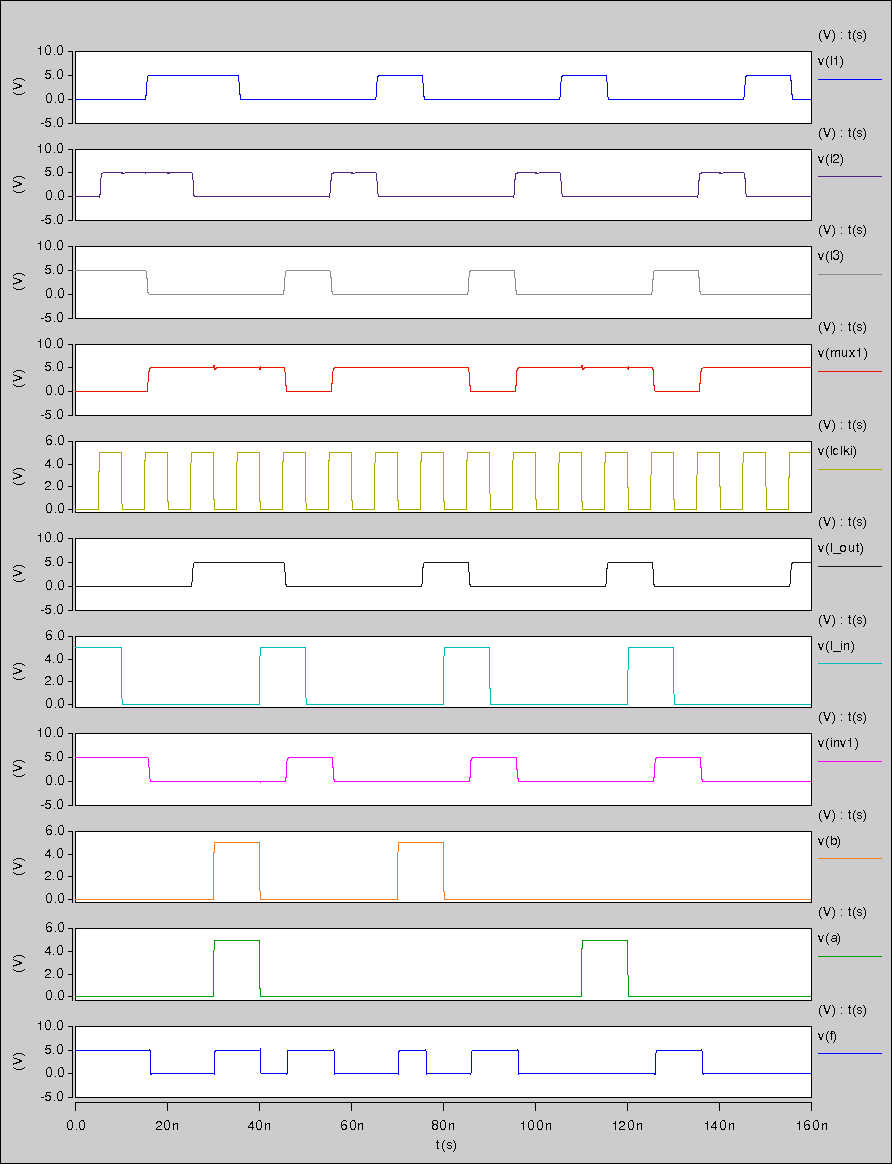
\includegraphics[width=\textwidth,height=\textheight,keepaspectratio]{../../cscope/lut_waveforms.png}
        \caption{\textbf{Hspice LUT Slice Wavefrom}}
        \label{fig:gg}
    \end{figure}

    \begin{figure}[H]
        \centering
        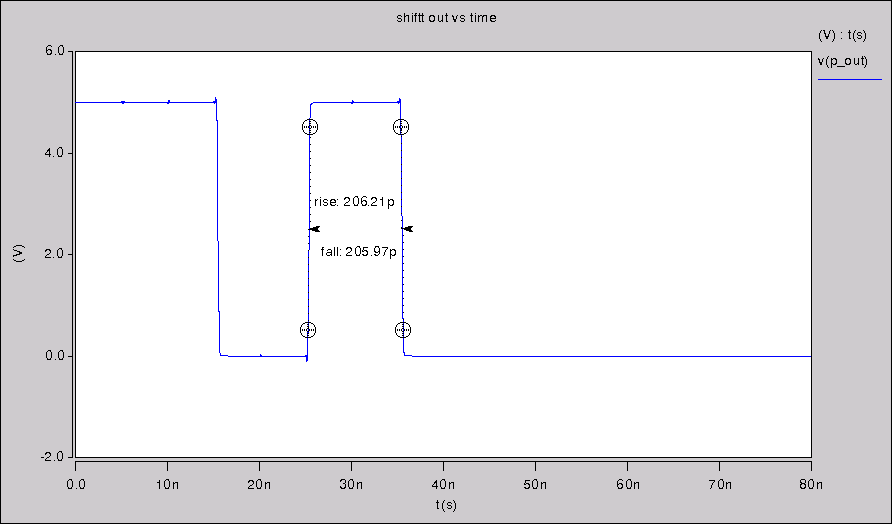
\includegraphics[width=\textwidth,height=\textheight,keepaspectratio]{../../cscope/shift_delay.png}
        \caption{\textbf{Hspice Delay of Shift Register Slice}}
        \label{fig:gg}
    \end{figure}
    \begin{figure}[H]
        \centering
        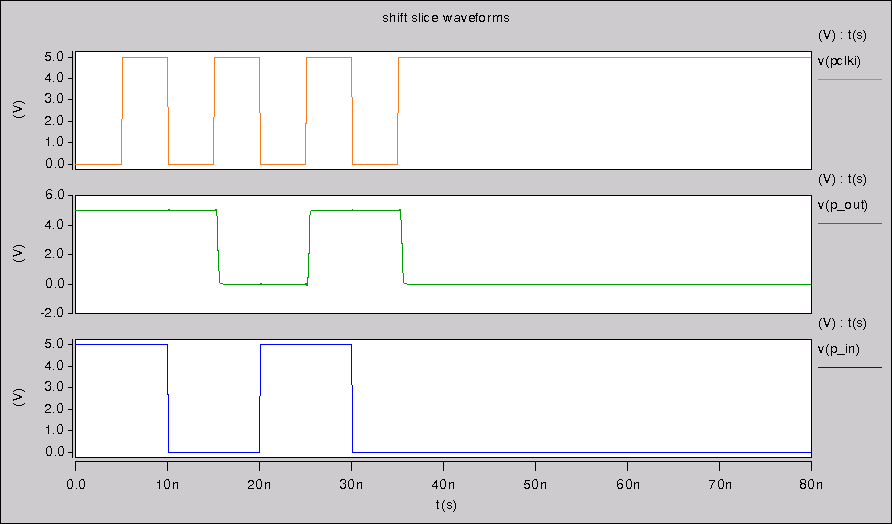
\includegraphics[width=\textwidth,height=\textheight,keepaspectratio]{../../cscope/shift_waveforms.png}
        \caption{\textbf{Hspice Shift Register Slice Waveform}}
        \label{fig:gg}
    \end{figure}

    %\newpage

\subsection{\textbf{Gate Level Simulations}}
    \begin{figure}[H]
        \centering
        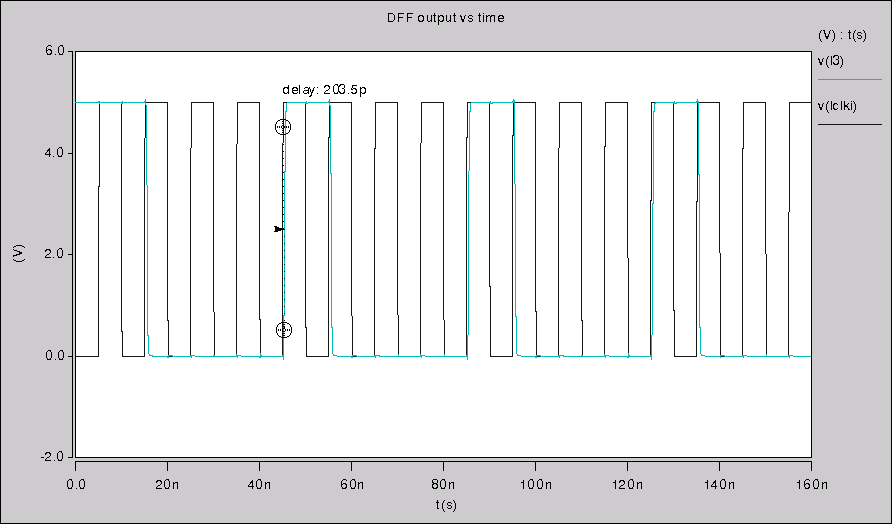
\includegraphics[width=\textwidth,height=\textheight,keepaspectratio]{../../cscope/dff_delay.png}
        \caption{\textbf{Hspice Delay of DFF}}
        \label{fig:gg}
    \end{figure}
    \begin{figure}[H]
        \centering
        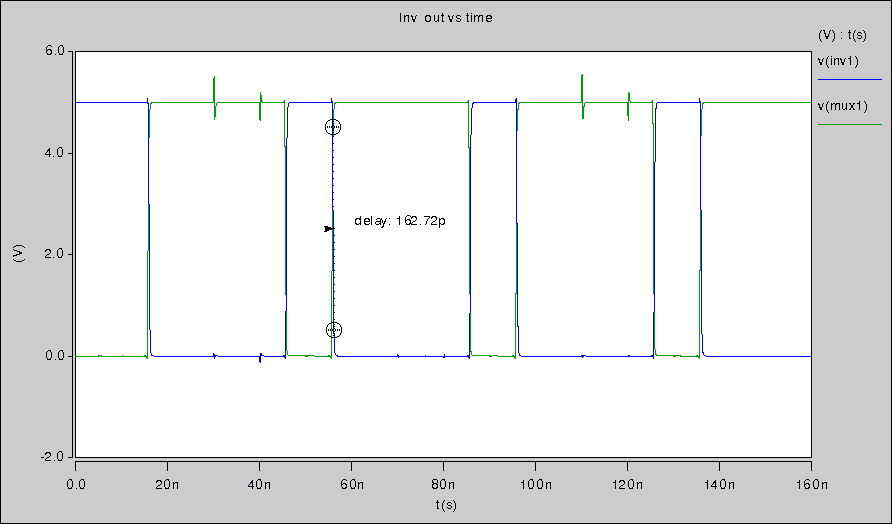
\includegraphics[width=\textwidth,height=\textheight,keepaspectratio]{../../cscope/inv1_delay.png}
        \caption{\textbf{Hspice Delay of Inveter}}
        \label{fig:gg}
    \end{figure}
    \begin{figure}[H]
        \centering
        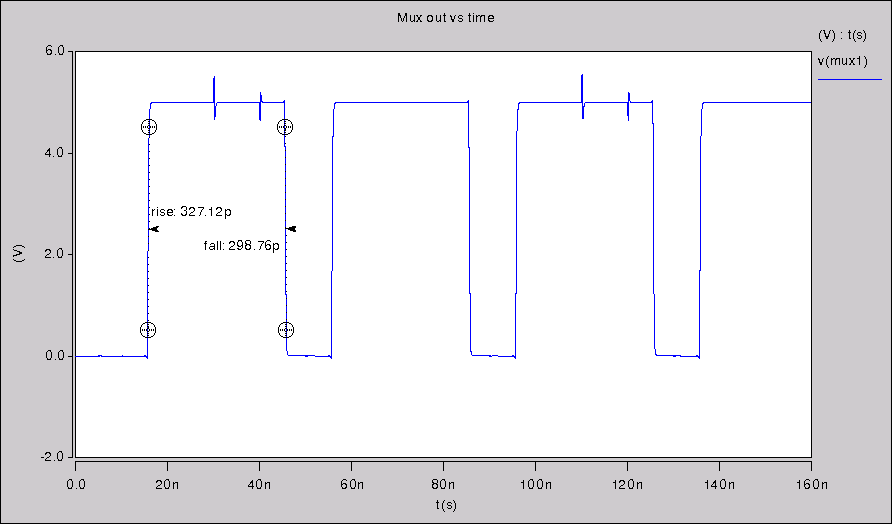
\includegraphics[width=\textwidth,height=\textheight,keepaspectratio]{../../cscope/mux1_delay.png}
        \caption{\textbf{Hspice Delay of Mux}}
        \label{fig:gg}
    \end{figure}

    \begin{table}[H]
        \centering
        \begin{tabular}{l | l | l | l}
            \hline
            &  \textbf{IRSIM}   & \textbf{VHDL} & \textbf{Hspice}\\ \hline
            \midrule
                Inverter    & 0.11 ns & 0.159 ns & 0.1627 ns \\
                Mux         & 0.315 ns & 0.312 ns &  0.31214 ns \\
                DFF         & 0.255 ns & 0.198 ns & 0.20305 ns \\
        \end{tabular}
        \caption{\textbf{Delay Times}}
    \end{table}

    \newpage

\section{\textbf{VHDL Modules with Delay}}

    \lstinputlisting[caption=\textbf{Top Module Delay}]{../../vhdl/top_del.vhd}
    \lstinputlisting[caption=\textbf{Look Up Table Module Delay}]{../../vhdl/lut_del.vhd}
    \lstinputlisting[caption=\textbf{Look Up Table Slice Module Delay}]{../../vhdl/lut_slice_del.vhd}

\subsection{\textbf{VHDL Test Bench Modules with Delay}}
    \lstinputlisting[caption=\textbf{Test Mode Enabled Test Bench}]{../../vhdl/top_test_del_tb.vhd}
    \lstinputlisting[caption=\textbf{Top Module Test Bench}]{../../vhdl/top_del_tb.vhd}

\subsection{\textbf{VHDL Gate Modules with Delay}}

    \lstinputlisting[caption=\textbf{DFF Module Delay}]{../../vhdl/dffposx1_del.vhd}
    \lstinputlisting[caption=\textbf{Inverter Module Delay}]{../../vhdl/invx1_del.vhd}
    \lstinputlisting[caption=\textbf{Inverter Module Delay}]{../../vhdl/mux2x1_del.vhd}

\section{\textbf{VHDL Modules Delay Waveforms}}
    \begin{figure}[H]
        \centering
        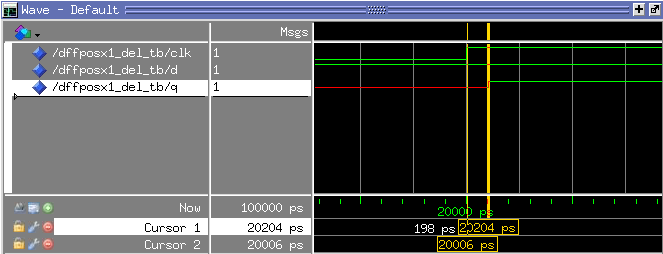
\includegraphics[width=\textwidth,height=\textheight,keepaspectratio]{../../vhdl/delay_waveforms/dff_delay.png}
        \caption{\textbf{Delay Waveform of DFF}}
        \label{fig:gg}
    \end{figure}
    \begin{figure}[H]
        \centering
        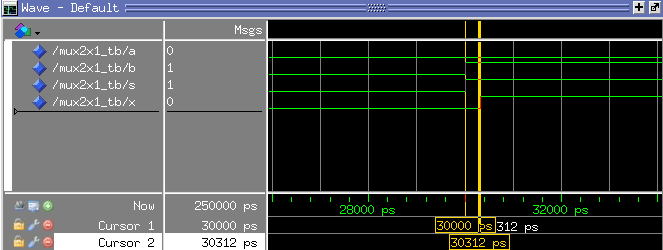
\includegraphics[width=\textwidth,height=\textheight,keepaspectratio]{../../vhdl/delay_waveforms/mux_delay.png}
        \caption{\textbf{Delay Waveform of MUX}}
        \label{fig:gg}
    \end{figure}
    \begin{figure}[H]
        \centering
        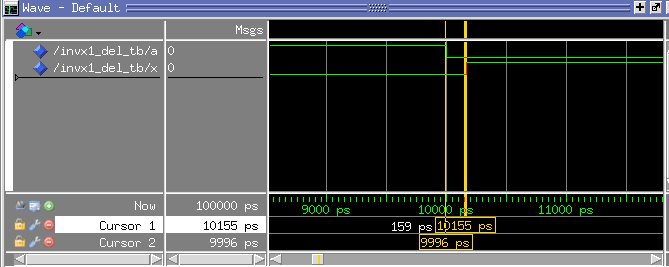
\includegraphics[width=\textwidth,height=\textheight,keepaspectratio]{../../vhdl/delay_waveforms/inv_delay.png}
        \caption{\textbf{Delay Waveform of Inverter}}
        \label{fig:gg}
    \end{figure}

    In table 4, we compare the delay results for each leaf level gate among the three design simulations.
    Please look at the figures listed above. We can see that these compare very well with each other. Also,
    note that in order to calculate the total delay time of the LUT slice, we must add up the delay values
    found from four D flip flops, three muxes, and three inverters. After adding them up, our LUT slice circuit
    gets a delay time of approximately {\raise.17ex\hbox{$\scriptstyle\sim$}}2 ns. Also, note that in order to get maximum clock rate, we just take
    the worst case delay of our circuit, and use this as a maximum clock rate. The table and figures above
    give us a worst case delay which is above the 50Mhz desirable signal.

    \begin{figure}[H]
        \centering
        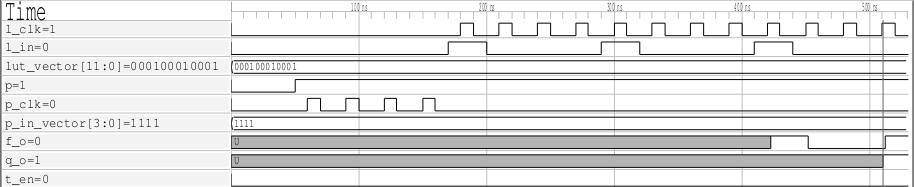
\includegraphics[width=\textwidth,height=\textheight,keepaspectratio]{../../vhdl/delay_waveforms/top_delay_wf.png}
        \caption{\textbf{Top Level Delay Waveform}}
        \label{fig:gg}
    \end{figure}
    \begin{figure}[H]
        \centering
        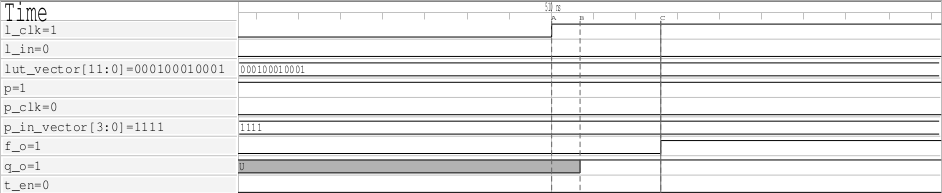
\includegraphics[width=\textwidth,height=\textheight,keepaspectratio]{../../vhdl/delay_waveforms/top_delay.png}
        \caption{\textbf{Top Level Delay Waveform Zoomed In}}
        \label{fig:gg}
    \end{figure}

    \begin{figure}[H]
        \centering
        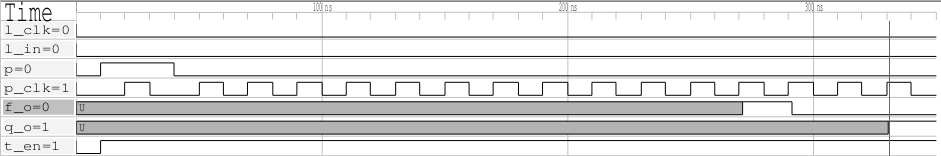
\includegraphics[width=\textwidth,height=\textheight,keepaspectratio]{../../vhdl/delay_waveforms/top_test_delay_wf.png}
        \caption{\textbf{Top Level Test Mode Enabled Delay Waveform}}
        \label{fig:gg}
    \end{figure}
    \begin{figure}[H]
        \centering
        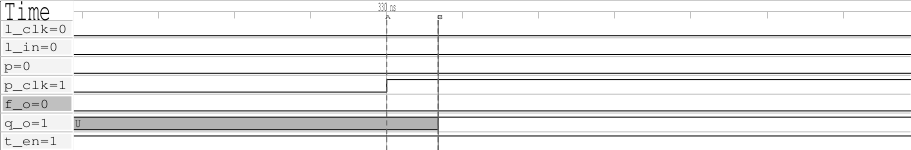
\includegraphics[width=\textwidth,height=\textheight,keepaspectratio]{../../vhdl/delay_waveforms/top_test_delay.png}
        \caption{\textbf{Top Level Test Mode Enabled Delay Waveform Zoomed In}}
        \label{fig:gg}
    \end{figure}

    As we can see here, the circuit still functions correctly given the delay times extracted from the
    simulations we have exhaustively gone through. This compares well with the previous simulation because
    as I have mentioned the functionality of the circuit still works properly. Also, we went ahead and measured
    the delay time for both the final Q and F output. In the above figure, the total delay time from A to B (Q
    output) was found to be 0.690 ns and from A to C (F output) was found to be {\raise.17ex\hbox{$\scriptstyle\sim$}}
    2.6 ns (worst case delay). This tells us that maximum clock speed achieved can be 1/2.6ns
    {\raise.17ex\hbox{$\scriptstyle\sim$}}384.6153846 MHz.

\section{\textbf{Floor Plan}}
    \begin{figure}[H]
        \centering
        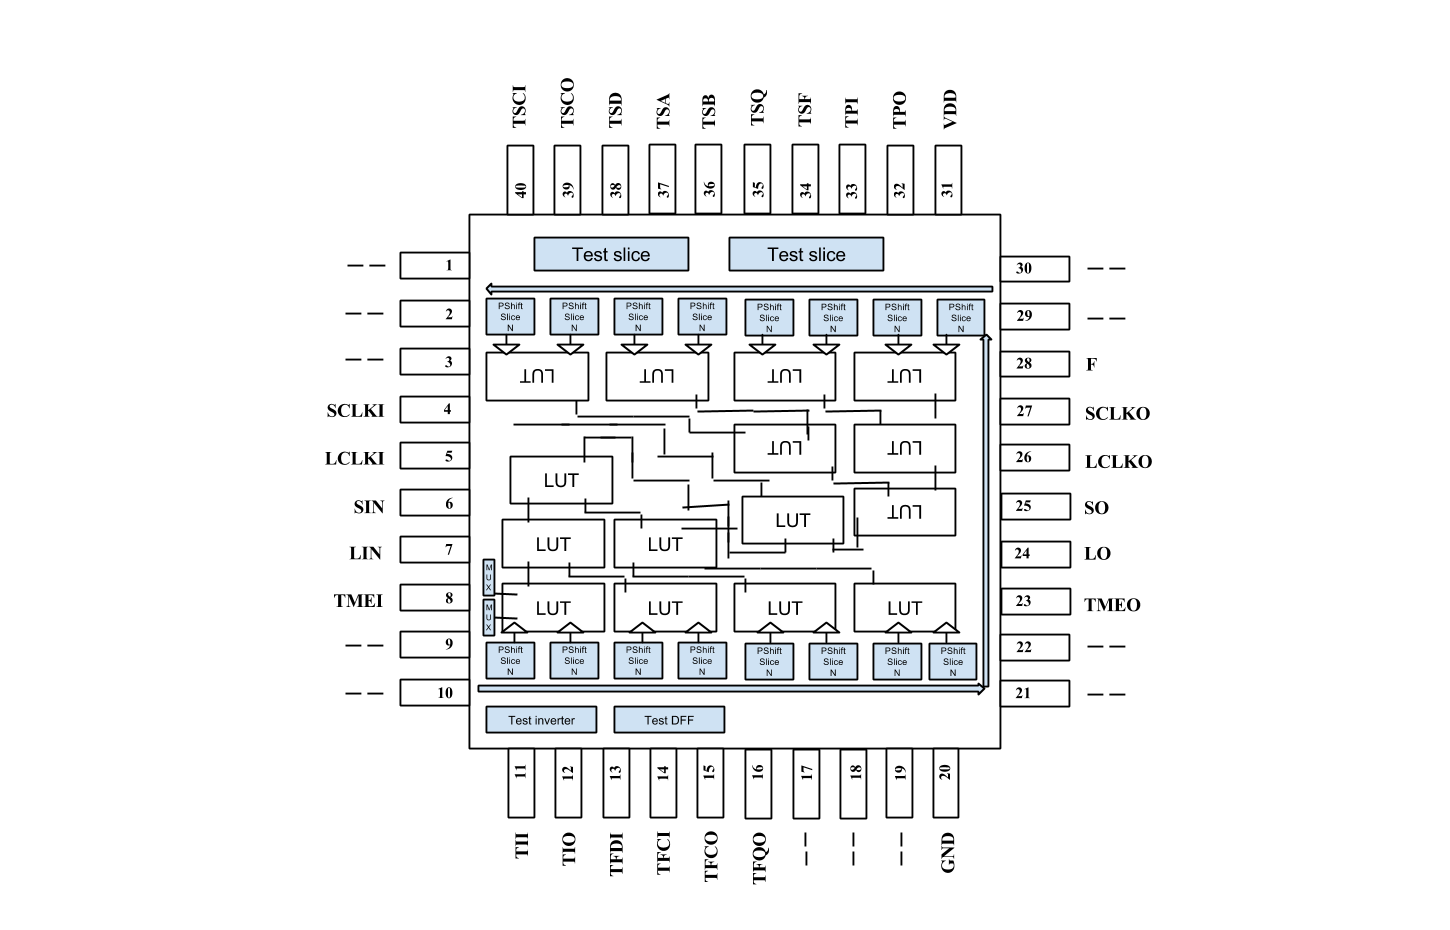
\includegraphics[width=\textwidth,height=\textheight,keepaspectratio]{../../floor_plan/floor_plan.png}
        \caption{\textbf{Floor Plan Design}}
        \label{fig:gg}
    \end{figure}

    This is the initial floor plan of our design. This is what we have come up with. It made it much easier
    for us to first design this floor plan in Magic and see how compact we can get it. The figure below shows
    the initial Magic Layout of the Chip. Below we can see that this is as compact as we can get it while at the
    same time we are able to fit 32 inputs for the shift register and 31 Look Up Tables.

    \begin{figure}[H]
        \centering
        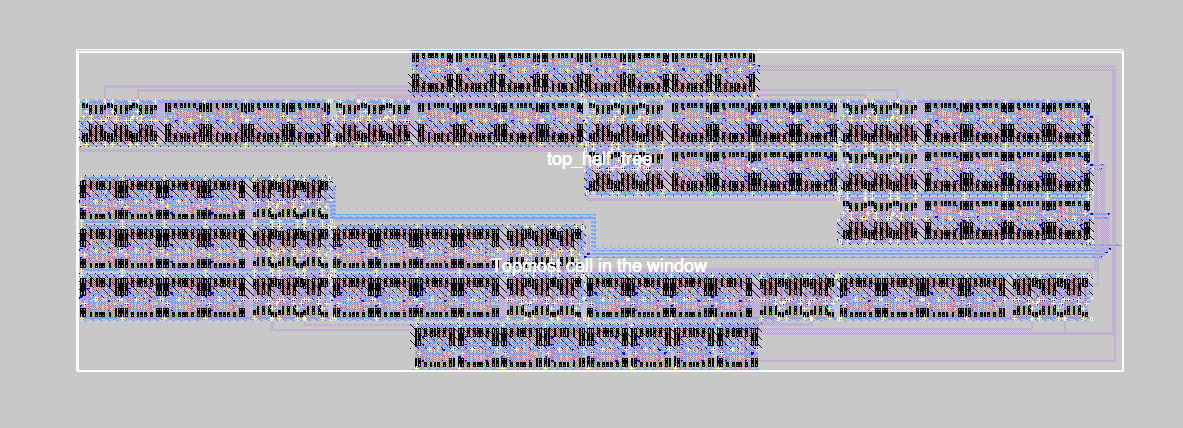
\includegraphics[width=\textwidth,height=\textheight,keepaspectratio]{../../magic/new_method/layout/initial_layout.png}
        \caption{\textbf{Initial Magic Layout Design}}
        \label{fig:gg}
    \end{figure}

\section{\textbf{Major Design Decisions}}
    We had to think of how to design our layout before we could come up with a floor plan. Since we have a binary
    tree, it was quite difficult to come up with an efficient way to utilize the whole area available given to us.
    Although we are not able to utilize all of the area provided, we came up with the most efficient way by
    stacking the LUTs together. At first, we thought we could fold the LUTs against each corner of the frame, but
    doing so, let to much wasted space in the middle. Another method we had in mind was to have all of the P shift
    registers to be stacked all the way around the edges, and have it go around in a spiral, but this was inefficient
    and made it difficult to connect. Therefore as you can see, the method we have come up with is shown in the figure below.
    This method makes it a bit more efficient and utilizes more space than what we have previously come up with.

\section{\textbf{Work Division}}
    \begin{table}[H]
        \centering
        \begin{tabular}{l | p{8cm}}
            \hline
            \textbf{Student}   & \textbf{Task} \\ \hline
            \midrule
                Both        & Modified Pin-out Diagram \\
                Both        & Magic Layout \\
                Both        & HSPICE \\
                Both        & IRSIM \\
                Both        & VHDL \\
                Both        & Floor Plan
        \end{tabular}
        \caption{\textbf{Task Assignment}}
    \end{table}
\end{document}
